\documentclass[11pt]{ctexart}

\usepackage{geometry}
\geometry{
    left = 0.6in,
    right = 0.6in,
    top = 0.8in,
    bottom = 1.0in
}
\usepackage{amssymb,amsbsy,amsmath,xcolor,mathrsfs,graphicx}
\usepackage{listings}
\usepackage{tasks}
\settasks{
    label = \Alph*. ,
    label-width = 16pt
}

\renewcommand{\title}[3]{
    \begin{center}
        \Large\heiti 中国电子学会 #1~年~#2~月 Python~#3级考试
    \end{center}
}
\newcommand{\TimeAndName}[1]{
    \begin{center}
        考试时间:~#1~ 分钟 \qquad\qquad\qquad\qquad 姓名:\underline{\quad\quad\quad\quad}
    \end{center}
}

\begin{document}
    \lstset{
        language = python,
        keywordstyle = \color{orange}\bfseries,
        emph = {
            abs, all, any, ascii, bin, bool, breakpoint, bytearray, bytes,
            callable, chr, classmethod, compile, complex, copyright, credits,
            delattr, dict, dir, divmod, enumerate, eval, exec, exit, filter,
            float, format, frozenset, getattr, globals, hasattr, hash,
            help, hex, id, input, int, isinstance, issubclass, iter, len,
            license, list, locals, map, max, memoryview, min, next, object,
            oct, open, ord, pow, print, property, quit, range, repr, reversed,
            round, set, setattr, slice, sorted, staticmethod, str, sum, super,
            tuple, type, vars, zip,
        },
        emphstyle = \color{purple}\bfseries,
        showspaces = false,
        basicstyle = \ttfamily,
        morekeywords = {True,False}
    }

    \title{2020}{6}{一}
    
    \TimeAndName{60}
    
    {\noindent\heiti 第一部分、单选题(共 25 题,每题 2 分,共50分.)}

    \begin{enumerate}
        % 1
        \item 以下哪种输入结果不可能得到反馈:{\heiti 重要的事情说三遍:安全第一!安全第一!安全第一!}?(\qquad)
        \begin{tasks}
            \task \lstinline{print("重要事情说三遍:" + "安全第一!" * 3)}
            \task \lstinline{print("重要事情说三遍:" + "安全第一!" + "安全第一!" * 2)}
            \task \lstinline{print("重要事情说三遍:" + "安全第一!" + "安全第一!" + "安全第一!")}
            \task \lstinline{print("重要事情说三遍:" + "安全第一!" / 3)}
        \end{tasks}

        % 2
        \item 执行 \lstinline{print(1 + 2 * 2 + 6 / 3)} 的结果为?(\qquad)
        \begin{tasks}(4)
            \task 4
            \task 7
            \task 4.0
            \task 7.0
        \end{tasks}

        % 3
        \item 已知变量 \lstinline{x=2},语句 \lstinline{print("x=", x)} 的作用是?(\qquad)
        \begin{tasks}(4)
            \task 在屏幕上输出 \lstinline{x=x}
            \task 在屏幕上输出 \lstinline{2=2}
            \task 在屏幕上输出 \lstinline{x=2}
            \task 在屏幕上输出 \lstinline{"x=2"}
        \end{tasks}

        % 4
        \item 执行如下程序后,画布上会出现几只海龟?(\qquad)
        \begin{lstlisting}
            import turtle
            t1 = turtle.Turtle("turtle")
            t2 = turtle.Turtle("turtle")
            t3 = turtle.Turtle("turtle")
            t4 = turtle.Turtle("turtle")
            t1.forward(50)
            t2.forward(100)
            t3.forward(150)
            t4.forward(200)
        \end{lstlisting}
        \begin{tasks}(4)
            \task 0
            \task 1
            \task 4
            \task 5
        \end{tasks}

        % 5
        \item \lstinline{print(24%5)} 的运算结果是?(\qquad)
        \begin{tasks}(4)
            \task 1
            \task 2
            \task 3
            \task 4
        \end{tasks}

        % 6
        \item 下面哪个指令不可以让海龟回到坐标$(0, 0)$点?(\qquad)
        \begin{tasks}(2)
            \task \lstinline{trutle.goto(0,0)}
            \task \lstinline{trutle.home()}
            \task \lstinline{turtle.setposition(0,0)}
            \task \lstinline{tutle.set(0,0)}
        \end{tasks}

        % 7
        \item 以下程序输出的结果是?(\qquad)
        \begin{lstlisting}
            a = 30
            b = 5
            print(a/b)
        \end{lstlisting}
        \begin{tasks}(4)
            \task 6
            \task 30/5
            \task 6.00
            \task 6.0
        \end{tasks}

        % 8
        \item \lstinline{print(46//8)} 的结果是?(\qquad)
        \begin{tasks}(4)
            \task 5
            \task 6
            \task 5.7
            \task 5.75
        \end{tasks}

        % 9
        \item Python 启动后显示的提示符是?(\qquad)
        \begin{tasks}(4)
            \task \lstinline{c:>}
            \task \lstinline{>>>}
            \task \lstinline{---}
            \task \lstinline{\%\%\%}
        \end{tasks}

        % 10
        \item 下列代码不能画出直径为 10 的点的是?(\qquad)
        \begin{tasks}(2)
            \task \lstinline{turtle.pensize(10)}\\
            \lstinline{trutle.pendown()}

            \task \lstinline{turtle.dot(10)}

            \task \lstinline{turtle.begin_fill()}\\
            \lstinline{turtle.circle(5)}\\
            \lstinline{turtle.end_fill()}

            \task \lstinline{turtle.begin_fill()}\\
            \lstinline{turtle.circle(10)}\\
            \lstinline{turtle.end_fill()}
        \end{tasks}

        % 11
        \item 运行下列程序后,绘制出以下哪个图形?(\qquad)
        \begin{lstlisting}
            import turtle
            turtle.pensize(3)
            turtle.forward(150)
            turtle.circle(50, 180)
            turtle.forward(180)
            turlte.circle(48, 180)
            turtle.forward(150)
            turtle.circle(45, 180)
            turtle.forward(120)
            turtle.done()
        \end{lstlisting}
        \begin{tasks}(4)
            \task 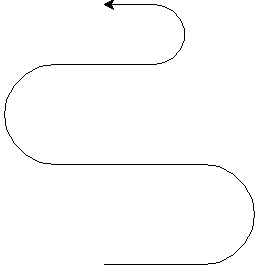
\includegraphics[width=.08\textwidth]{11a.png}
            \task 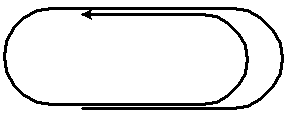
\includegraphics[width=.12\textwidth]{11b.png}
            \task 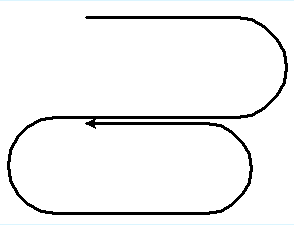
\includegraphics[width=.12\textwidth]{11c.png}
            \task 
\includegraphics[width=.12\textwidth]{11d.png}
        \end{tasks}

        % 12
        \item 已知变量 \lstinline{a = 5}, \lstinline{b = 6},执行语句 \lstinline{a *= a + b} 后,变量 \lstinline{a} 的值为?(\qquad)
        \begin{tasks}(4)
            \task 11
            \task 30
            \task 31
            \task 55
        \end{tasks}

        \newpage
        % 13
        \item 如果 \lstinline{a = 23}, \lstinline{b = 10},那么 \lstinline{print(a%b)} 的结果是?(\qquad)
        \begin{tasks}(4)
            \task 2
            \task 3
            \task 23
            \task 2.3
        \end{tasks}

        % 14
        \item 下列表达式的值为 \lstinline{True} 的是?(\qquad)
        \begin{tasks}(4)
            \task \lstinline{'a' > 'b'}
            \task \lstinline{2 > 3}
            \task \lstinline{'A' > 'a'}
            \task \lstinline{'3' > '2'}
        \end{tasks}
        
        % 15
        \item 已知 \lstinline{x = 5}, \lstinline{y = 6}, 表达式 \lstinline{not(x != y)} 的值为?(\qquad)
        \begin{tasks}(4)
            \task \lstinline{True}
            \task \lstinline{False}
            \task 5
            \task 6
        \end{tasks}

        % 16
        \item 输出如下古诗,请问哪句是正确的?(\qquad)
        \begin{lstlisting}
            闻道梅花坼晓风,雪堆遍满四山中。
            何方可化身千亿,一树梅花一放翁。
        \end{lstlisting}
        \begin{tasks}
            \task \lstinline{print(}\\
            \lstinline{'闻道梅花坼晓风,雪堆遍满四山中。}\\
            \lstinline{何方可化身千亿,一树梅花一放翁。')}

            \task \lstinline{print('闻道梅花坼晓风,雪堆遍满四山中。'}\\
            \lstinline{'何方可化身千亿,一树梅花一放翁。')}

            \task \lstinline{print(\'\'\'闻道梅花坼晓风,雪堆遍满四山中。}\\
            \lstinline{何方可化身千亿,一树梅花一放翁。\'\'\')}

            \task \lstinline{print("闻道梅花坼晓风,雪堆遍满四山中。"\\n}\\
            \lstinline{"何方可化身千亿,一树梅花一放翁。")}
        \end{tasks}

        % 17
        \item 执行以下两段代码结果?(\qquad)
        \begin{lstlisting}
            a = 123
            print(a % 100 % 10)
        \end{lstlisting}
        \begin{tasks}(4)
            \task 1
            \task 2
            \task 3
            \task 1.23
        \end{tasks}

        % 18
        \item 下面描述中,不符合 Python 语言特点的是?(\qquad)
        \begin{tasks}(2)
            \task Python 是一门面向对象的编程语言
            \task Python 程序通过编译后运行
            \task Python 支持函数编程
            \task Python 支持多个操作系统
        \end{tasks}

        % 19
        \item 下列哪个不是 Python 的保留字?(\qquad)
        \begin{tasks}(4)
            \task if
            \task or
            \task do
            \task for
        \end{tasks}

        \newpage
        % 20
        \item 下面代码的结果是?(\qquad)
        \begin{lstlisting}
            a = 5
            print('a + 4')
        \end{lstlisting}
        \begin{tasks}(4)
            \task 9
            \task \lstinline{'a + 4'}
            \task 无结果,出错
            \task \lstinline{a + 4}
        \end{tasks}

        % 21
        \item 在 \lstinline{turtle} 库中的执行,执行以下代码指令后,走出的一个正方形形状,此时海龟的面朝方向应该是往哪里?(\qquad)(4)
        
        \begin{minipage}{.53\textwidth}
            \begin{lstlisting}
                import turtle
                turtle.goto(0,0)
                turtle.goto(0, 100)
                turtle.goto(100 ,100)
                turtle.goto(100 ,0)
                turtle.goto(0, 0)
            \end{lstlisting}
        \end{minipage}
        \begin{minipage}{.4\textwidth}
            \begin{tasks}
                \task 水平向左
                \task 水平向右
                \task 垂直向上
                \task 垂直向下
            \end{tasks}
        \end{minipage}     

        % 22
        \item 执行下列语句后的结果是什么?(\qquad)
        \begin{lstlisting}
            b = 2 * a / 4
            a = 1
            print(a, b)
        \end{lstlisting}
        \begin{tasks}(4)
            \task \lstinline{1, 0.5}
            \task \lstinline{1, 0}
            \task 报错
            \task \lstinline{0, 1}
        \end{tasks}

        % 23
        \item 执行下面程序后,以下哪个图形是正确的?(\qquad)
        
        \begin{minipage}{.53\textwidth}
            \begin{lstlisting}
                import turtle
                turtle.shape('square')
                turtle.home()
                turtle.dot()
                turtle.stamp()
                turtle.forward(100)
                turtle.setheading(90)
                turtle.stamp()
                turtle.forward(100)
                turtle.left(90)
                turtle.stamp()
                turtle.forward(100)
                turtle.left(90)
                turtle.stamp()
                turtle.forward(100)
            \end{lstlisting}
        \end{minipage}
        \begin{minipage}{.4\textwidth}
            \begin{tasks}
                \task 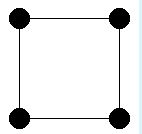
\includegraphics[width=.2\textwidth]{23a.png}
                \task 
\includegraphics[width=.2\textwidth]{23b.png}
                \task 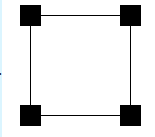
\includegraphics[width=.2\textwidth]{23c.png}
                \task 
\includegraphics[width=.2\textwidth]{23d.png}
            \end{tasks}
        \end{minipage}   

        % 24
        \item 下面哪个程序,最后可能得到右侧图形 
\includegraphics[width=.05\textwidth]{24.png}?(\qquad)
        \begin{tasks}(2)
            \task \lstinline{turtle.setheading(0)}\\
            \lstinline{turtle.circle(50, 90)}\\
            \lstinline{turtle.circle(-50, -90)}\\
            \lstinline{turtle.circle(50, 90)}\\
            \lstinline{turtle.circle(-50, -90)}

            \task \lstinline{turtle.setheading(-180)}\\
            \lstinline{turtle.circle(50, 90)}\\
            \lstinline{turtle.circle(-50, -90)}\\
            \lstinline{turtle.circle(-50, -90)}\\
            \lstinline{turtle.circle(50, 90)}

            \task \lstinline{turtle.setheading(90)}\\
            \lstinline{turtle.circle(50, 90)}\\
            \lstinline{turtle.circle(50, 90)}\\
            \lstinline{turtle.circle(-50, -90)}\\
            \lstinline{turtle.circle(-50, -90)}

            \task \lstinline{turtle.setheading(270)}\\
            \lstinline{turtle.circle(-50, -90)}\\
            \lstinline{turtle.circle(50, 90)}\\
            \lstinline{turtle.circle(50, 90)}\\
            \lstinline{turtle.circle(-50, -90)}
        \end{tasks}

        % 25
        \item 以下选项中,Python 语言中代码注释使用的符号是?(\qquad)
        \begin{tasks}(4)
            \task \lstinline{/... .../}
            \task \lstinline{!}
            \task \lstinline{\#}
            \task \lstinline{//}
        \end{tasks}
    \end{enumerate}

    {\noindent\heiti 第二部分、判断题(共 10 题,每题 2 分,共20分.)}
    \begin{enumerate}
        \setcounter{enumi}{25}
        % 26
        \item \lstinline{print()} 函数不可以在屏幕上打印出空行.(\qquad)

        %27
        \item Turtle 库中,使用 \lstinline{circle(20)} 命令,指的是画出以画布正中央为圆心,半径为 20 的圆形.(\qquad)
        
        %28
        \item 在 IDLE 编辑器中,Python 代码的字体和字号可以根据需要自行设置,方便大家的使用.(\qquad)
  
        %29
        \item \lstinline{Abc}、\lstinline{aBc}、\lstinline{abC} 是三个不同的变量.(\qquad)
        
        %30
        \item 以下程序的运行结果是 9.(\qquad)
        \begin{lstlisting}
            one, two, three = '1', 3, 5
            print(one + two + three)
        \end{lstlisting}
        
        %31
        \item \lstinline{a *= b} 等价于 \lstinline{a = b * b}.(\qquad)
        
        %32
        \item Python 除了用自带的 IDLE 编程外,还可以用其他编程环境进行程序编写,比如 JupyterNotebook.(\qquad)
        
        %33
        \item \lstinline{turtle.circle(50, steps=5)} 命令可以画出一个五角星.(\qquad)
        
        %34
        \item \verb|is| 和 \verb|input| 都是关键字,不能随意用. (\qquad)
        
        %35
        \item 下面语句的显示结果是 \lstinline{a b}.(\qquad)
        \begin{lstlisting}
            print("a", end=" ")
            print("b", end=" ")
        \end{lstlisting}
    \end{enumerate}

    \newpage
    {\noindent\heiti 第三部分、编程题(共 2 题,共30分.)}
    \begin{enumerate}
        \setcounter{enumi}{35}
        
        % 36
        \item 绘制图形:
        \begin{tasks}[label = (\arabic*)]
            \task 绘制出如下图的图形,两根线段长度为 200 且互相垂直,圆的直径为 200;
            \task 圆的中心位置为画布中心,即两根线段的交点;
            \task 画笔宽度为 2,颜色为红色.
        \end{tasks}
        \begin{center}
            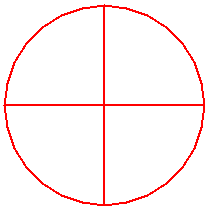
\includegraphics[width=.2\textwidth]{36.png}
        \end{center}
        \vfill

        %37
        \item 牛奶重量:
        
        已知一头奶牛每天可以产 20 千克牛奶,问 $N$ 头奶牛 7 天可以产多少千克牛奶?
        \begin{tasks}[label = (\arabic*)]
            \task 程序开始后,会给出提示字符串:“请输入奶牛的头数:”,完成奶牛的输入;
            \task 程序会根据输入的奶牛头数计算出总共产出的牛奶的重量,并将结果进行修饰然后输出。示例:如果输入奶牛的头数为10,则输出“\textcolor{red}{10 头奶牛7天可以产 1400 千克的牛奶}”.
        \end{tasks}
        \vfill
    \end{enumerate}
\end{document}